\section{需求工程过程}

\subsection{概述}
过程是一组相关活动的集成,通过这些活动的执行,可以完成一项任务或者达到一个目标。

需求工程过程是系统开发当中需求开发活动的集成,它的模版是产生一个能够在用户环境下解决用户业务问题的系统方案。

需求工程过程可能会表现出极大的差异,但是除了少数情况之外,主要的需求工程活动是比较固定的。

\begin{figure}[H]
	\setcounter{subfigure}{0}
	\centering
	\vspace{-0.5em}	
	\subfloat{
	\begin{minipage}[c]{0.4\linewidth}
	\centering
	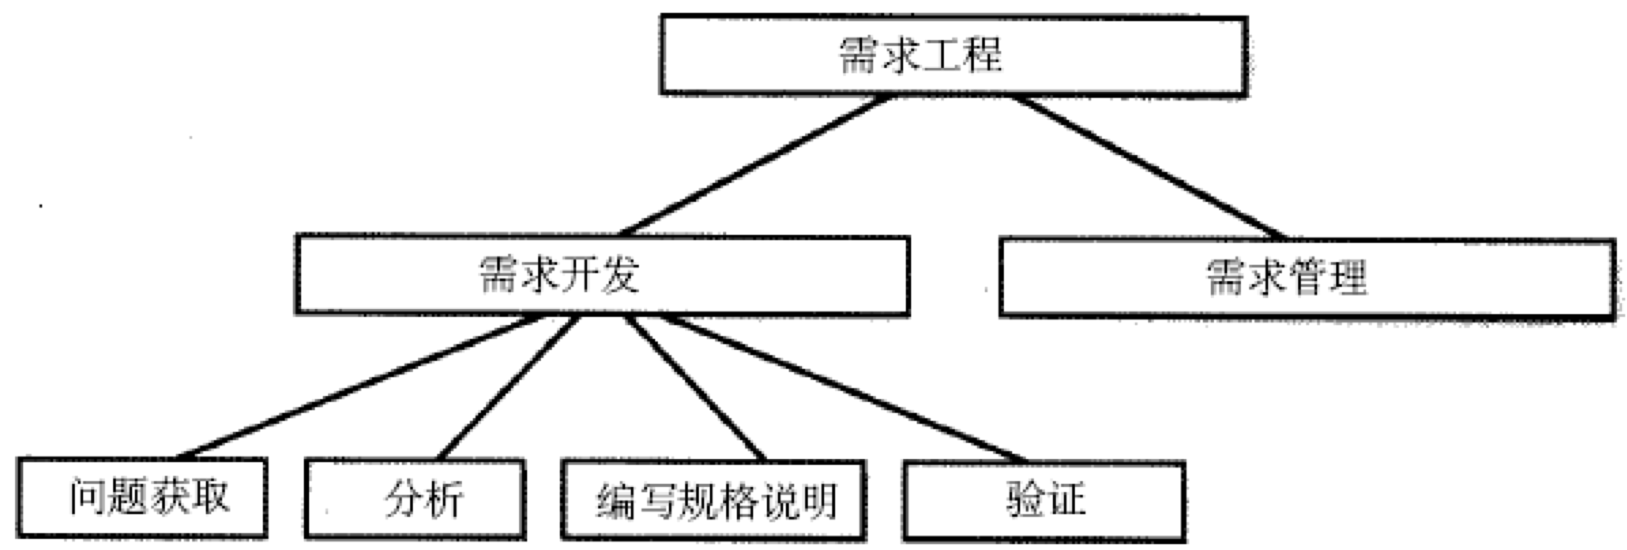
\includegraphics[width=\linewidth]{img/需求工程过程1.png}
	\end{minipage}
    }
	\subfloat{
	\begin{minipage}[c]{0.57\linewidth}
	\centering
	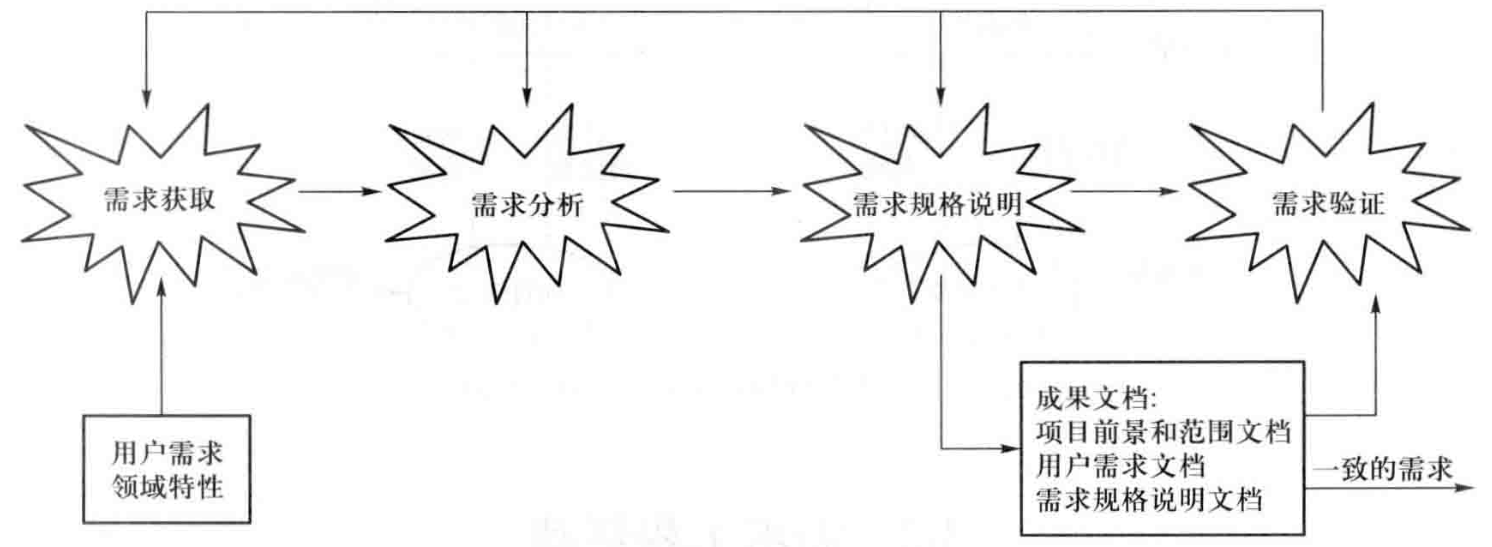
\includegraphics[width=\linewidth]{img/需求工程过程2.png}
	\end{minipage}
	}
	\centering
	\vspace{-1em}
\end{figure}

\subsection{需求工程的基本活动}
\begin{itemize}
    \item \textbf{需求获取:}系统原始需要
    \begin{itemize}
        \item 研究应用环境,分析系统涉众,了解已有问题,建立系统目标,获取业务细节,生成用户需求
    \end{itemize}
    \item \textbf{需求分析:}保证需求完整性与一致性(贯穿整个过程)
    \begin{itemize}
        \item 将目标、功能与约束映射为系统行为,建立系统模型并分析(信息的细化与隐藏联系、假设的显式化),识别并修复不一致缺陷,发现并弥补遗漏的需求
    \end{itemize}
    \item \textbf{需求规约:}将分析过的需求与系统行为明确并文档化
    \begin{itemize}
        \item 自然语言$+$模型语言(UML)
    \end{itemize}
    \item \textbf{需求验证:}保证需求分档的正确性、一致性、完整性
    \begin{itemize}
        \item 最终产物为所有涉众一致同意的需求规约,是后续开发的基础
    \end{itemize}
    \item \textbf{需求管理:}持续(时间、开发活动)管理需求基线
    \begin{itemize}
        \item 跟踪后续阶段中的需求实现与变更,确保正确的理解与实现
    \end{itemize}
\end{itemize}

\subsection{需求开发过程是迭代和并发的}
\begin{figure}[H]
	\setcounter{subfigure}{0}
	\centering
	\vspace{-2em}	
	\subfloat{
	\begin{minipage}[c]{0.48\linewidth}
	\centering
	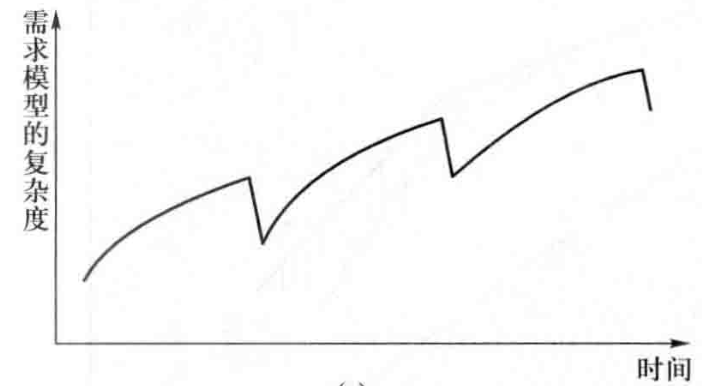
\includegraphics[width=0.8\linewidth]{img/需求开发过程是迭代和并发的1.png}
	\end{minipage}
    }
	\subfloat{
	\begin{minipage}[c]{0.48\linewidth}
	\centering
	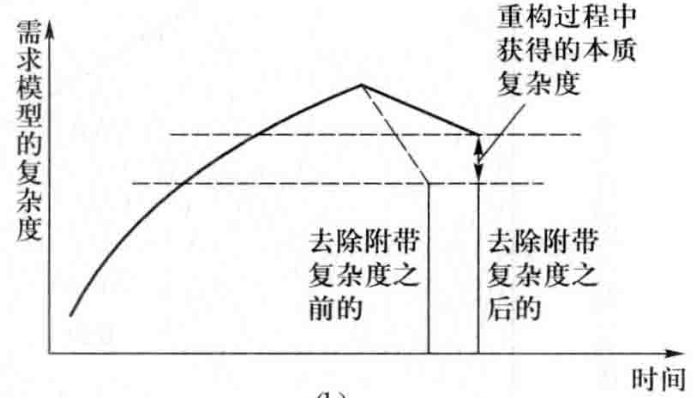
\includegraphics[width=0.8\linewidth]{img/需求开发过程是迭代和并发的2.png}
	\end{minipage}
	}

    \subfloat{
        \begin{minipage}[c]{0.55\linewidth}
        \centering
        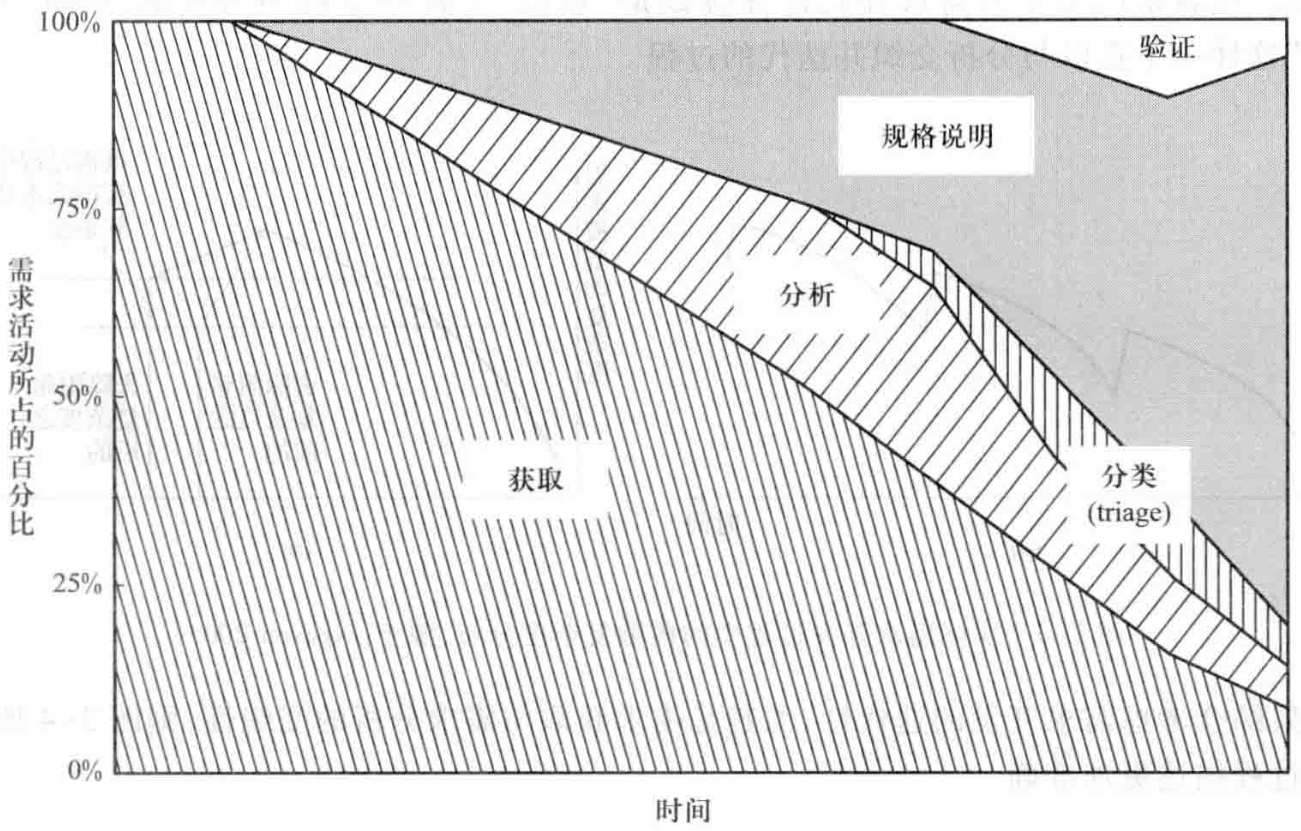
\includegraphics[width=0.97\linewidth]{img/需求开发过程是迭代和并发的3.png}
        \end{minipage}
    }
	\centering
	\vspace{-1em}
\end{figure}


\subsection{实践方法的应用}

\vspace{-0.8em}
\begin{center}
    \begin{longtable}{|m{2cm}|m{3.5cm}|m{3.2cm}|m{4.6cm}|}
        \hline
        \multicolumn{1}{|c|}{活动} & \multicolumn{1}{c|}{有效实践}   & \multicolumn{1}{c|}{内容}          & \multicolumn{1}{c|}{技术及方法}                \\ \hline
        \multirow{15}{*}{需求获取}   & 定义项目前景                      & 定义项目前景                           & 问题分析、目标分析、业务过程分析、分析非功能需求、定义系统边界、编写前景与范围文档 \\ \cline{2-4} 
                                 & 控制项目范围                      & 控制项目范围                           & 同上                                        \\ \cline{2-4} 
                                 & \multirow{3}{*}{实现用户价值}     & 涉众识别                             & 先膨胀后收缩、检查列表、涉众网络                          \\ \cline{3-4} 
                                 &                             & 涉众描述                             & 涉众的描述特征                                   \\ \cline{3-4} 
                                 &                             & 涉众评估                             & 优先级评估、风险评估、共赢分析                           \\ \cline{2-4} 
                                 & \multirow{2}{*}{促进用户参与}     & 涉众代表选择                           & 代表采样、使用用户替代源                              \\ \cline{3-4} 
                                 &                             & 参与策略制定                           & 制定参与基本策略、敏捷方法---用户参与                      \\ \cline{2-4} 
                                 & \multirow{3}{*}{识别并使用各种需求源} & 涉众分析                             & 涉众分析的各种方法(如前述)                            \\ \cline{3-4} 
                                 &                             & 硬数据采样                            & 硬数据采样                                     \\ \cline{3-4} 
                                 &                             & 需求重用                             &                                           \\ \cline{2-4} 
                                 & \multirow{4}{*}{有效的获取需求}    & 建立有效交流机制                         & 建立合作关系,维护交流气氛,利用适当的交流途径、交流方式              \\ \cline{3-4} 
                                 &                             & \multirow{3}{*}{\begin{tabular}[c]{@{}l@{}}正确使用需求获取\\ 方法\end{tabular}}      & 面谈/调查问卷/群体面谈、头脑风暴                         \\ \cline{4-4} 
                                 &                             &                                  & 原型                                        \\ \cline{4-4} 
                                 &                             &                                  & 观察、民族志、文档分析/需求重用/需求剥离                     \\ \cline{2-4} 
                                 & 收集和组织需求获取的结果                & 建立收集和组织需求结果的机制                   & 用例/场景模型                                   \\ \hline
        \multirow{6}{*}{需求分析}    & \multirow{3}{*}{为需求建模}      & \multirow{2}{*}{\begin{tabular}[c]{@{}l@{}}通过建模手段明确和\\理解需求信息\end{tabular}} & 结构化分析模型                                   \\ \cline{4-4} 
                                 &                             &                                  & 面向对象分析模型                                  \\ \cline{3-4} 
                                 &                             & 使用多种手段从多角度建模相同的内容                & 多视点方法、Wieringa框架、Zachman框架                \\ \cline{2-4} 
                                 & 在合适的层次上描述需求                 & 需求细化                             &                                           \\ \cline{2-4} 
                                 & 唯一地标识每一条需求                  & 需求细化                             &                                           \\ \cline{2-4} 
                                 & 划分需求的优先级                    & 确定需求优先级                          & 累计投票、区域划分、Top-N、数据量化                      \\ \hline
        \multirow{4}{*}{需求规格说明}  & 使用模板                        & 使用需求文档模板                         & {[}IEEE 1998{]}的模板                        \\ \cline{2-4} 
                                 & \multirow{3}{*}{进行良好的写作}    & 综合使用各种描述手段                       & 形式化、半形式和非形式化描述                            \\ \cline{3-4} 
                                 &                             & \multirow{2}{*}{学习有效的写作实践}       & 写作技巧、优秀需求规格说明文档特性                         \\ \cline{4-4} 
                                 &                             &                                  & 需求写作事项、优秀需求的特性                            \\ \hline
        需求验证                     & 验证需求                        & 使用有效方法进行需求的验证和确认                 & 需求评审、原型与模拟、开发测试用例、用户手册编制、利用跟踪关系、自动化分析     \\ \hline
        \multirow{3}{*}{需求管理}    & 建立和维护需求基线                   & 建立和维护需求基线                        & 配置管理、状态维护                                 \\ \cline{2-4} 
                                 & 进行变更控制                      & 进行变更控制                           & 变更控制过程、变更控制事项(策略)                         \\ \cline{2-4} 
                                 & 建立需求跟踪信息                    & 建立需求跟踪信息                         & 低端/高端的需求跟踪使用、需求依赖                         \\ \hline
    \end{longtable}
\end{center}
\vspace{-3.7em}


